%%
%% sample document for AAMAS'18 conference
%%
%% modified from sample-sigconf.tex
%%
%% see ACM instructions acmguide.pdf
%%
%% AAMAS-specific questions? n.yorke-smith@tudelft.nl
%%

\documentclass[sigconf]{aamas}  % do not change this line!

%% your usepackages here, for example:
\usepackage{booktabs}
\newcommand{\specialcell}[2][c]{%
	\begin{tabular}[#1]{@{}c@{}}#2\end{tabular}}
\usepackage{dirtytalk}
\usepackage{enumitem}
\usepackage{blindtext}
\usepackage{multirow}
\usepackage{booktabs}
\usepackage{graphicx}
\usepackage{stfloats}
%% do not change the following lines
%% do not change the following lines
\setcopyright{ifaamas}  % do not change this line!
\acmDOI{doi}  % do not change this line!
\acmISBN{}  % do not change this line!
\acmConference[AAMAS'19]{Proc.\@ of the 18th International Conference on Autonomous Agents and Multiagent Systems (AAMAS 2019), N.~Agmon, M.~E.~Taylor, E.~Elkind, M.~Veloso (eds.)}{May 2019}{Montreal, Canada}  % do not change this line!
\acmYear{2019}  % do not change this line!
\copyrightyear{2019}  % do not change this line!
\acmPrice{}  % do not change this line!
%% the rest of your preamble here


%%%%%%%%%%%%%%%%%%%%%%%%%%%%%%%%%%%%%%%%%%%%%%%%%%%%%%%%%%%%%%%%%%%%%%%%%%%%%%%%%%%%%%%%%%%%%%%%%%%%%%%%%

\begin{document}

%\title{Towards Analyzing Theory of Mind from Public Attitude Survey Data using POMDP}
%\title{Towards Analyzing Theory of Mind from a Public Attitude Survey Data generated POMDP}
%\title{Towards Analyzing Human Behavior from a Public Attitude Survey using Machine Generated POMDP}
%\title{Towards an Automated Construction of Decision-Theoretic Models of Human Behavior} % put your title here!
\title{Automated Construction of Human Behavior Models Using Correlation Analysis}
%\titlenote{Produces the permission block, and copyright information}

% AAMAS: as appropriate, uncomment one subtitle line; check the CFP
%\subtitle{Extended Abstract}
%\subtitle{Industrial Applications Track}
%\subtitle{Socially Interactive Agents Track}
%\subtitle{Blue Sky Ideas Track}
%\subtitle{Robotics Track}
%\subtitle{JAAMAS Track}
%\subtitle{Doctoral Mentoring Program}

%\subtitlenote{The full version of the author's guide is available as \texttt{acmart.pdf} document}


% AAMAS: submissions are anonymous for most tracks
\author{Paper \#XXX}  % put your paper number here!

%% example of author block for camera ready version of accepted papers: don't use for anonymous submissions
%
%\author{Ben Trovato}
%\authornote{Dr.~Trovato insisted his name be first.}
%\orcid{1234-5678-9012}
%\affiliation{%
%  \institution{Institute for Clarity in Documentation}
%  \streetaddress{P.O. Box 1212}
%  \city{Dublin}
%  \state{Ohio}
%  \postcode{43017-6221}
%}
%\email{trovato@corporation.com}
%
%\author{G.K.M. Tobin}
%\authornote{The secretary disavows any knowledge of this author's actions.}
%\affiliation{%
%  \institution{Institute for Clarity in Documentation}
%  \streetaddress{P.O. Box 1212}
%  \city{Dublin}
%  \state{Ohio}
%  \postcode{43017-6221}
%}
%\email{webmaster@marysville-ohio.com}
%
%\author{Lars Th{\o}rv{\"a}ld}
%\authornote{This author is the
%  one who did all the really hard work.}
%\affiliation{%
%  \institution{The Th{\o}rv{\"a}ld Group}
%  \streetaddress{1 Th{\o}rv{\"a}ld Circle}
%  \city{Hekla}
%  \country{Iceland}}
%\email{larst@affiliation.org}
%
%\author{Valerie B\'eranger}
%\affiliation{%
%  \institution{Inria Paris-Rocquencourt}
%  \city{Rocquencourt}
%  \country{France}
%}
%\author{Aparna Patel}
%\affiliation{%
% \institution{Rajiv Gandhi University}
% \streetaddress{Rono-Hills}
% \city{Doimukh}
% \state{Arunachal Pradesh}
% \country{India}}
%\author{Huifen Chan}
%\affiliation{%
%  \institution{Tsinghua University}
%  \streetaddress{30 Shuangqing Rd}
%  \city{Haidian Qu}
%  \state{Beijing Shi}
%  \country{China}
%}
%
%\author{Charles Palmer}
%\affiliation{%
%  \institution{Palmer Research Laboratories}
%  \streetaddress{8600 Datapoint Drive}
%  \city{San Antonio}
%  \state{Texas}
%  \postcode{78229}}
%\email{cpalmer@prl.com}
%
%\author{John Smith}
%\affiliation{\institution{The Th{\o}rv{\"a}ld Group}}
%\email{jsmith@affiliation.org}
%
%\author{Julius P.~Kumquat}
%\affiliation{\institution{The Kumquat Consortium}}
%\email{jpkumquat@consortium.net}
%
%% The example's default list of authors is too long for headers
%\renewcommand{\shortauthors}{B. Trovato et al.}


\begin{abstract}  % put your abstract here!
Decision-theoretic agents have shown potential in modeling and simulating human behavior across many scenarios of importance to decision-makers. Unfortunately, constructing such models manually, even when informed by social science, is a time-consuming and error-prone process. In contrast, it is very easy to apply correlation analysis to human-behavior data, but the resulting statistical correlations do not necessarily support a causal model for the simulations of interest. In this work, we implement and evaluate a method for leveraging statistical correlation in the automated construction of decision-theoretic models of human behavior. In particular, we analyze survey data from Afrobarometer across multiple countries and years to identify significant correlations among the variables. We translate these variables into components of a Partially Observable Markov Decision Process (POMDP) and the correlations among them into the transition probabilities among these variables. The resulting POMDPs are simulation objects that we can evaluate by comparing their decisions against those of the people surveyed. We verify our design by comparing how well it scales to different subsets of the problem space. We validate the results by comparing it against both a simple baseline and the survey outcomes themselves.
\end{abstract}


% AAMAS: the ACM CCS are not needed within AAMAS papers
%%
%% The code below should be generated by the tool at
%% http://dl.acm.org/ccs.cfm
%% Please copy and paste the code instead of the example below.
%%
%\begin{CCSXML}
%<ccs2012>
% <concept>
%  <concept_id>10010520.10010553.10010562</concept_id>
%  <concept_desc>Computer systems organization~Embedded systems</concept_desc>
%  <concept_significance>500</concept_significance>
% </concept>
% <concept>
%  <concept_id>10010520.10010575.10010755</concept_id>
%  <concept_desc>Computer systems organization~Redundancy</concept_desc>
%  <concept_significance>300</concept_significance>
% </concept>
% <concept>
%  <concept_id>10010520.10010553.10010554</concept_id>
%  <concept_desc>Computer systems organization~Robotics</concept_desc>
%  <concept_significance>100</concept_significance>
% </concept>
% <concept>
%  <concept_id>10003033.10003083.10003095</concept_id>
%  <concept_desc>Networks~Network reliability</concept_desc>
%  <concept_significance>100</concept_significance>
% </concept>
%</ccs2012>
%\end{CCSXML}
%
%\ccsdesc[500]{Computer systems organization~Embedded systems}
%\ccsdesc[300]{Computer systems organization~Redundancy}
%\ccsdesc{Computer systems organization~Robotics}
%\ccsdesc[100]{Networks~Network reliability}


\keywords{AAMAS; ACM proceedings; POMDPs; Human Behavior Models; Multiagent Social Simulation}  % put your semicolon-separated keywords here!

\maketitle


%%%%%%%%%%%%%%%%%%%%%%%%%%%%%%%%%%%%%%%%%%%%%%%%%%%%%%%%%%%%%%%%%%%%%%%%%%%%%%%%%%%%%%%%%%%%%%%%%%%%%%%%%
%% start of main body of paper

\section{Introduction}



Human behavior models can provide modeling assistance for behavioral studies. It can assist in sociology studies with applications in policy making and disaster relief scenarios. 

However there is lack of techniques in generating behavior models in an automated fashion. Dynamics of decision making and human behavior can be very complex. Macrosociology and microsociology studies can be concerned with complex dynamics of individuals or groups which can be difficult to model correctly. When constructing a behavior model most of the design choices are left to human interpretation and decision making. Such design choices can introduce human bias in the model design. 

Moreover creating a behavior model manually can be labor intensive, hence it limits the complexity of the dynamics which can decrease the effectiveness of the model. Depending on the implementation, the number of dynamics required to represent N states and M actions can be of $N\cdot M$, that is if there is a relationship between each state and action. To determine and calculate the actions' effects on a state, it can require additional decision making and analysis. To generate the dynamics for only 10 states and 10 actions would require 100 decisions by a model maker. A mistake or bias in any of those 100 decisions will in turn be introduced to the final behavior model design. 

For our study we focused on generating a behavior model which encapsulates multiple POMDP models. We used public attitude survey data and an automated approach to generate the dynamics for that model. Public attitude survey data can take large efforts to collect and span over long time periods. Such data can have a wealth of information on the behavior of individuals and groups represented by the survey. A POMDP can model the uncertainty in the dynamics of our society inherently. A multiagent system can then be used to model and study individuals or groups of survey participants.
 
Questions in survey data can be abstract and make it difficult to generate well-defined mappings to POMDP dynamics. The dynamics generated manually can lack the complexity to encapsulate the interactions of different agents. The reliable mapping of the survey data and a POMDP is not a trivial task.
 
There are works that introduce Machine Generated POMDPs [], however such models require manual effort in the design choices. A set of design choices required would be modeling the agent and environment interaction, modeling effect of actions on each state, reward function, nature of agent which we discuss later in Section[2.1]. Public attitude surveys can be sparse, go through changes in their method of collecting the data. Often times preprocessing the data is not enough as we explain at Section \ref{sec:generatingdynamics}. Behavior model objectives and outcomes can also differ from such Machine Generated POMDPs, the data can lack the structure to train such a model. Such Machine Generated POMDPs, require human intervention to some extent to fit the training data and so increases manual effort in modeling. Increase in manual effort to generate the dynamics will in turn induce bias or mistakes in design choices.

 %There are other works that use correlation and traditional statistical analysis techniques in analyzing public attitude survey data[]. 

Other works examine human behavior by manually generating POMDPs[]. While previous works have introduced semi-automated techniques in generating such POMDPs[]. In our work we introduce a behavior model by which we can increase the degree of freedom in generating POMDPs. 

There are decision-theoretic framework that introduce quantitative modeling of multiple agents [PsychSim]. Such frameworks create a layer of abstraction between the POMDP dynamics and the behavior model. This in turn as shown by [Semi-structured] can improve the efficiency of designing the model by eliminating the search of the entire problem space.

\textbf{TODO: Finish references}
\section{MODEL DESIGN}

We wish to build a social-simulation model that reflects the decision making process of individuals and groups based on survey data. To that end, we construct a behavior model that encapsulates a POMDP. In precise terms, a POMDP is defined as a tuple {$ \mathbf{\langle S, A, P, \Omega, O, R \rangle }$. Our work utilizes a multiagent POMDP framework PsychSim []. We build on top of other works that introduce semi-automated approaches at constructing behavior models such as that of Pynadath et al.[AAMAS2016]. In each of the following subsections, we detail the abstractions and problem relaxations that this model design introduces to enable the automated construction of a human behavior model.

We evaluate our design by modeling after Afrobarometer, a public attitude survey which focuses on African countries. We considered survey data from 2003 to 2013. The survey includes information about the participants Socioeconomic characteristics, beliefs, and  events in their community. The survey data had to be pre-processed due to erroneous values, spelling mistakes and re-coding of available answers between different survey rounds.

Due to the structure of survey data, it is often not possible to generate a POMDP directly without any manual effort. We have reduced the amount of manual effort required by our design to only identifying the attributes that we want to study in our model and their sentiment. This manual effort includes identifying \textbf{Actions} that the agents can take, \textbf{Dynamic States} that those agents hold and \textbf{Static States} that describe those agents. For each Action and Dynamic State identified, the sentiment scale of the responses needs to be identified as Neutral to Positive/Negative. The sentiments and responses for each question require a manual recoding process. Each response has a sentiment strength that is utilized to decide the priority over states. We also had to identify  each Dynamic State and Action as Maximizing or Minimizing. 

\subsection{Agent}

The Agent is the \textit{Subject} of the study. It is reasonable to create multiple agents when designing a behavior model. Common social dynamics involve multiple actors. Such actors can be simulated based on game-theoretic scenarios. Information about the interactions of agents is not always available and hence encapsulating this into our model design makes it difficult.

An \textbf{Introspective Agent Model} observes and interacts only with itself as well as its objective states. The agent's actions, states and rewards encapsulate the behaviors of other social entities that relate to the agent we are studying without having to model all of the interaction dynamics explicitly. In order to accomplish this objective, we infer the actions and states of relevant external social entities and consider the total sum of effects from these outside factors on our agent. The effects are then aggregated and abstracted by this single agent.

\subsection{States}

In our model design, we distinguish the states into two categories: \textbf{dynamic states} and \textbf{static states}. 


Based on which aspect of an Agent we are studying, we select a set of questions as the quantities of interest and we treat them as dynamic states or static states. In some cases we want to control by the Age, Tribe, Nationality of a survey participant. 




\subsubsection{Dynamic States}\label{sec:dynamicstates}
Dynamic States are the dependent variables of the simulation which can change over time. In our model, these states encapsulate the agent's beliefs about the operating environment and satisfy different objectives. They also serve as goals whose values the agent wants to minimize or maximize. These states' quantities are the byproduct of what we want to study, which is the decision making of an agent. 

To avoid bias in the actions agents take, we set the change function for each dynamic state as an approximation function. 
\textbf{TODO mathematical representation of approximation function} In a behavior model, similar to real world dynamics, the Dynamic State can reach saturation. After taking a certain action, the change of the value of a dynamic state is proportional to both the weight of that particular action-dynamic state as well as the distance of the current state value to its optimal value.

Consider the following dynamic state:

\say{\textbf{Q18B. Over the past year, how often, if ever, have you or anyone in your family: Feared crime in your own home?}}

\begin{description}
	\item [1] Never
	\item [2] Just once or twice
	\item [3] Several times
	\item [4] Many Times
	\item [5] Always
\end{description} 

We can use the response from this question to identify the strength of the sentiment towards that dynamic state. We create a dynamic state which is the perception of crime. A response with stronger sentiment, has a higher initial value for that dynamic state. The initial value of dynamic states when modeling groups is the mean value of the sentiment strength normalized. Sentiment strength and its calculation are described in section \ref{sec:generatingdynamics}.

\subsubsection{Static States}
Static States do not change over the course of the simulation. They are the conditional variables independent of the dynamics of the simulation for which we choose static states so we can control the experiment. For the purposes of our model, static variables represent the agent's identity. 

Questions we considered as static states included ones observed by the interviewer directly or can hold an objective truth. Such questions include identifying information for the participant such as Country, Gender, Tribe. 

Consider the following question by which we chose to control our experiment.

\textbf{What is your ethnic community, cultural group or tribe?}

This question has 2760 unique answers between participants of all survey rounds and countries. 

\subsection{Actions}



The actions of an Agent can be directly deducted from the data we are modeling or inferred by it. We are inferring an action from the data by the change in the Agent's belief states. While we can't observe the action directly we can study its effects. We are concluding that if there is a \textit{Goal Actor} - our Subject - there must be another Agent acting upon it. 

At that extend we extract the actions of survey participants directly or infer them. A sample of question from which we can directly infer the action is the following:
\say{\textbf{Q26. With regard to the most recent national election in [20xx], which statement is true for you?}}

We can also indirectly infer the actions from questions like Q19B.

\say{\textbf{Q19B. During the past year, have you or anyone in your family been physically attacked?}}

In this case, both the Attacker and Subject of the action are part of the same group that we are modeling. It is unlikely that the attacker belongs to a different Country. The choice of inferred actions highly depends on the Static States we choose to control our experiment by. The direct link between the attacker's behavior, action and effect are missing. For such questions we utilize an \textit{Introspective Agent} that on one hand represents the victim while on the other hand encapsulates the attackers that change the agent's own states. Hence, the agent encapsulates both the attacker and the victim. The effects of those actions and corresponding probability distributions are inferred from the survey we are studying. 

\subsection{Transition Probability} 


Transition probability in a POMDP model represents the probabilistic effects of an action on the world states. It is an essential part of the modeling task because it is used in an agent's bounded look-ahead process to determine the value for each candidate action, similar to the mental process of how people evaluate the consequences of their decisions. 


Information regarding the effects of an action taken by a person is not directly observable from public survey data. Survey data focuses on human social behaviors and not on the causal relationships between different social behaviors. Determining the Transition Probability between each mental process is important in creating a Human Behavior Model. Therefore, we regard modeling such relationship as the core of our modeling tasks.

We conform to standard POMDP's use of Dynamic Bayesian networks and influence diagrams exploit conditional independence in modeling the effects of actions. We thus are able to express the dependencies between effects and actions as links between nodes in a dynamic influence diagram. To further reduce the elicitation of expert knowledge in the mapping of effects with actions we use correlation analysis to determine pairs of states and actions whose dependencies are statistically significant. We determine the impact of actions on states by the strength of the correlation. We examine each question individually with each other question using spearman correlation. The correlation value is then used to generate the weight of each question that represents an action to a question that represents a dynamic state.A positive correlation value corresponds to an action maximizing the value of that dynamic state, while a negative correlation is minimizing.

The POMDP is then solved for a given horizon distance and the reward value $V(b,a_w)$ of each action $a_w$ for each belief state $b$ is calculated. Instead of having our agents choose an action with the maximum reward value we evaluate the soft max over the rewards of all possible actions to calculate the respective probability an agent is likely to pick an action. Hence an iteration of our model returns 

\begin{equation}
\pi(b)=\frac{e^{r*V(b,a_w)}}{\sum_{a\epsilon A} e^{r* V(b,a)}} \forall a_w\epsilon A
\end{equation}

Consider as an example for our survey, after we solve the POMDP model, our outcomes are in the form of a list of actions inferred from the survey questions and the probability an individual will choose to take that action.We also study the impact of an action to a belief state explained in \textbf{Section[]}. An example of a set of actions into study are 'Q15.Employment', 'Q26.Voted', 'Q25C.Demonstration', 'Q25D. Refused', 'Q25A.Meeting', 'Q25B.RaiseIssue', 'Q19A.Stolen', 'Q19B.Attacked'. Each action is maximizing or minimizing in context of a dynamic state depending on the correlation of the state and action.

\subsection{Observations}

$\Omega$  is  a  set  of  possible  observations  that  the  agent  may receive. $O$ is the probability of receiving specific observations given the current state of the world. An observation can be used to update the agent's belief state with new information and study how their perspectives of the world change in relation to the actual transition of the world.

Due to the limited information from the survey data we can't model observations directly. We consider all states to be fully observable. Here an observation indicates the current time stamp. If the sentiment strength towards a question determines the observation at the time. For example, a strong sentiment towards the dynamic state mentioned in \textbf{Section[2.2.1]} Q18B, fear of crime, is suggestive of someone being victim to a crime recently. The time difference between different rounds of interviews can  be a few years and require a new model to be build. There are external factors that are not possible to be encapsulated in our model from the data available. Such external factors could be political, religious unrest or even natural disaster. In addition, modeling observations with the data available from public attitude surveys can be problematic in studying large group dynamics as opposed to more granular agents.

In our survey we partially consider observations in the modeling of Dynamic States. During the sentiment recoding process of the survey responses \textbf{Incomplete!}

%%%%%%%%%%%%%%%%%%%%%%%


\subsection{Rewards}

The reward objective is to minimize or maximize a Dynamic State. The semantic meaning of the survey questions is used in determining the reward of that action to a Dynamic State.

Consider two questions which encapsulate a Dynamic State that an agent would want to maximize and minimize respectively:

\say{\textbf{Q11B. In general, how would you describe your own living conditions?}}

Living conditions is something that someone would want to improve, \textit{maximize}. 

\say{\textbf{Q16A. Over the past year, how often, if ever, have you or anyone in your family gone without enough food to eat?}}

Lack of food on the other hand is a dynamic state an agent would like to \textit{minimize}. 

We model Rewards from the data as the priority weight for the Dynamic States. We determine the exact values based on the sentiment scores on each response. Responses with extreme sentiments can be seen as higher priority to the agent we model. Determining the sentiment scale requires recoding of the responses.

For a typical survey question in the data we studied the sentiment scale doesn't require recoding. The question is simply asking degree of agreement or disagreement. Responses in this instance would include:

\begin{description}
	\item [1] Strongly Disagree
	\item [2] Mildly Disagree
	\item [3] neither disagree nor agree
	\item [4] mildly agree
	\item [5] Strongly Agree
\end{description} 


In other cases the questions carry a negative sentiment, the response scale has to be inverted. Consider the question with responses:

\say{Q16A. Over the past year, how often, if ever, have you or anyone in your family gone without enough food to eat?}

"Never" in this case is regarded as the neutral response while "Always" is the strongest sentiment response.

Denial to respond or lack of a response are also recorded in the survey we studied. In such cases there is a response but is declining to respond as opposed to a missing response. All such responses are recoded as neutral responses. 

Having a correct sentiment scale we calculate the mean response value for each question within the population subjects we study. A response with stronger sentiment would naturally be a higher priority than a response with a lower sentiment score. Therefore, we designate as reward weights the sentiment score of each question after we normally distribute them. 


\section{DATA MODELING}

In this section we explain the process by which we convert the survey data into a Human Behavior Model. Our approach utilizes a correlation analysis to identify the link between actions and dynamic states. If this process was done by hand, it would require N*M number of informed decisions where N is the number of actions and M the number of states. For a simple model, there are 10 actions and 10 dynamic states. A domain expert would need to make 100 informed decisions about the connection of each action to a state. The domain expert would also need to determine if an action will have a positive effect on a state, a negative effect, and what is the effect of that action to that state. All of this would require either manual analysis or intuition in the process of generating the dynamics. 

Moreover such a model would need to be build for each individual represented by the survey. Making larger scale analysis impossible. We reduce this manual effort that can be prone to bias, by calculating the correlation. Additionally we introduce a granular model by which we can generate dynamics for by representing multiple participants with a single model or as granular as a single participant.

\subsection{Data Processing}


To avoid bias by over-represented questions in our dataset, we find highly correlated questions and we aggregate them. In a public survey, many questions can be expressing the same concept or the different aspects of one fact or social phenomenon. Considering them as separate actions or separate states in the dynamics of our model can skew the decision of the agent to certain actions due to the stochastic nature of the POMDP. To reduce this risk, we use spearman's correlation to determine how well a group of variables can be described using the same function or quantity. We group them into a dynamic state if these variables stand for states, or otherwise aggregate the effects of their action into one action. We chose a correlation coefficient $\rho>0.8$ and a confidence interval $p<0.05$.  

\textbf{TODO change graph to separate beliefs and actions}
Consider Figure \ref{fig:corrmapall}, multiple groups of questions have high correlation either positive or negative. That is partly because questions have the same semantic meaning so the answers and sentiment towards those questions is highly correlated for our given data sample. After aggregating highly correlated questions the corresponding correlation map can be seen at Figure \ref{fig:cormapprocess}



We removed noise for the correlation analysis from missing questions by discarding the missing responses for that specific question when calculating the correlation for that specific agent. We don't discard the entire respondent's response because doing so yields a significant smaller population sample that doesn't allow a model to be build. Missing values in large scale surveys are common. 

After having defined the dynamic states, actions, and sentiment of each action, we are able to generate the dynamics which describe the Human Behavior Model. We calculate the correlation coefficient between all questions we are considering, both as actions and dynamic states. We then proceed by merging the effects of questions that have highly correlated responses. Highly correlated questions can often be survey questions that contain the same semantic meaning.  



\begin{figure}[H]
	\centering
	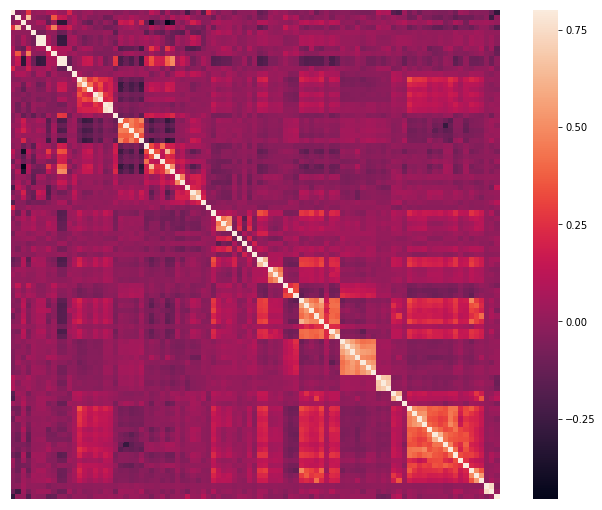
\includegraphics[width=0.7\linewidth]{Images/corrmap_all}
	\caption{Correlation Map of All questions}
	\label{fig:corrmapall}
\end{figure}

\begin{figure}[H]
	\centering
	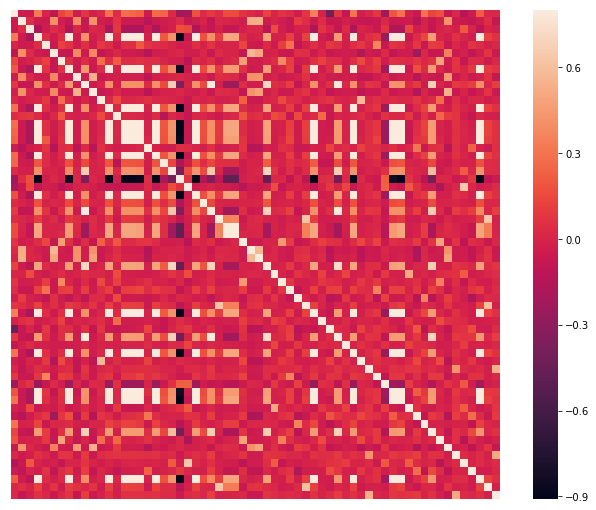
\includegraphics[width=0.7\linewidth]{Images/cormap_processed.png}
	\caption{Correlation Map after processing}
	\label{fig:cormapprocess}
\end{figure}


Consider the questions: 

\say{\textbf{Q24A. Have you attended a community meeting during the past year. If not, would you do if you had the chance?}}


\say{\textbf{Q25B. Have you got together with others to raise an issue during the past year. If not, would you do if you had the chance?}}


For some participants the responses were identical in terms of sentiment strength, because the questions are semantically the same to many participants. For such questions we choose to aggregate the effects to reduce the noise during the execution of a POMDP. This is done to avoid the bias that such dynamic states would introduce to actions. 

The same process is applied for actions. This is done to reduce the bias multiple actions with the same semantic meaning have on the POMDP.



\subsection{Dynamics Construction}


\subsection{Model Granularity}

With our model design we can represent a single survey participant or group following the same rules for generating the model. Moreover we can adjust the level of granularity we want to use based on how well the model fits that participant group. Instead of performing an exhaustive problem space search, we can use the currently generated model dynamics to generate new dynamics for more or less granular agents. A more granular agent will contain more Static States and Dynamic States as well as more complex dynamics and mapping between the actions and the Dynamic States. 

Less granular representation of the agent and the dynamics on the other hand aggregates the effects of multiple states and their dynamics. A less granular model in consequence has less control variables or Static States and represents a bigger number of survey participants.

We can choose to control granularity for this specific dataset by considering responses such as Gender, Age Group and more.


\subsection{Agent Execution}

The POMDP model encapsulates the decision making process by computing the expected reward, \(E[R]\), of each candidate action in \(A\). Because we aim our model as an agent to simulate the social behaviors of the typical individuals in a given population, we set our model's initial states as mean values of the answers to corresponding survey questions within this population. We then have the model calculate the values for candidate actions by applying the transition probability and reward functions. After the action values are generated, instead of singling out the action with maximal value, we wish to obtain a probability distribution that reveals the chance of an agent taking each candidate action respectively. Thus, we use a \textit{softmax} to calculate this probability distribution as described in Eqn[1]. We make the likelihood of each action choice dependent on its corresponding action value. 

\textbf{TODO: Insert necessary math formulas}

The resulting distribution of the action choice generated can then be compared to that in the survey data for model evaluation. 


\begin{figure*}[t!]
	\centering 
	
	\caption{Probability Distributions for Bottom Up evaluation}
	\begin{minipage}
		{0.32\textwidth}
		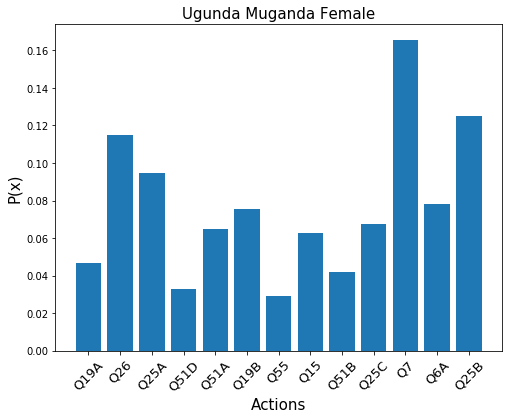
\includegraphics[width=\linewidth]{Images/UgundaMugandaFemaleTopDownHDM.png}
		\label{fig:ugundamugandafemaletopdown}
	\end{minipage}\hfill
	\begin{minipage}{0.32\textwidth}%
		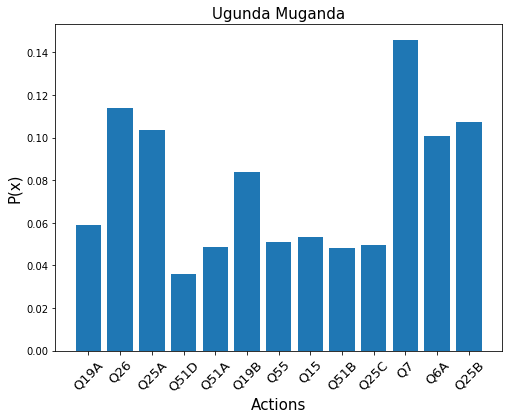
\includegraphics[width=\linewidth]{Images/UgundaMugandaTopDownHDM.png}
		\label{fig:ugundamugandatopdown}
	\end{minipage}\hfill
	\begin{minipage}{0.32\textwidth}
		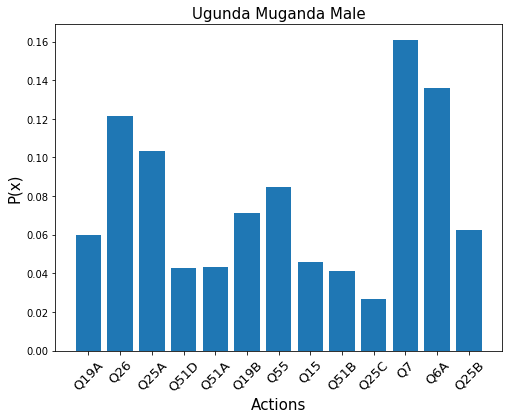
\includegraphics[width=\linewidth]{Images/UgundaMugandaMaleTopDownHDM.png}
		\label{fig:ugundamugandamaletopdown}
	\end{minipage}
	
	\caption{Probability Distributions for Top Down evaluation}
	\begin{minipage}
		{0.32\textwidth}
		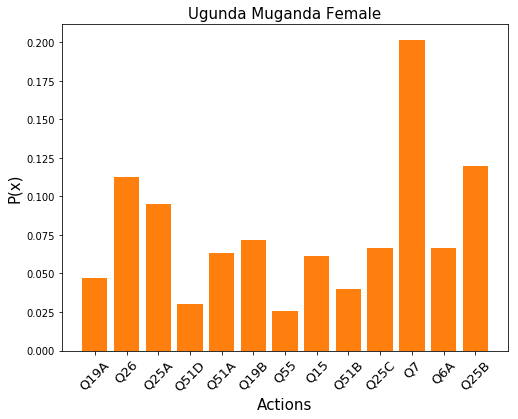
\includegraphics[width=\linewidth]{Images/botomupfemale.png}
		\label{fig:ugundamugandafemalebottomup}
	\end{minipage}\hfill
	\begin{minipage}{0.32\textwidth}
		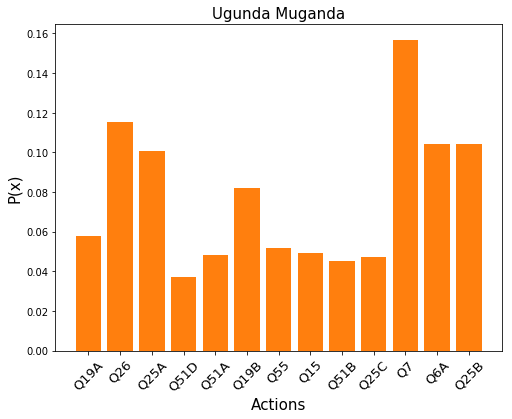
\includegraphics[width=\linewidth]{Images/bottomup.png}
		\label{fig:ugundamugandamalebottomup}
	\end{minipage}\hfill
	\begin{minipage}{0.32\textwidth}%
		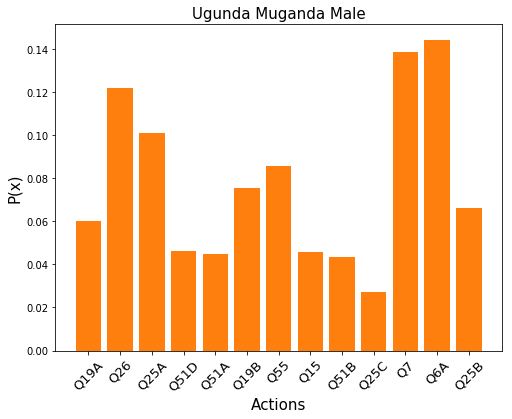
\includegraphics[width=\linewidth]{Images/botomupmale.png}
		\label{fig:ugundamugandabottomup}
	\end{minipage}
\end{figure*}



\section{EXPERIMENTS}


For the purposes of this empirical evaluation we perform our experiments on a subgroup of survey participants from the tribe of Muganda in Ugunda between the years 2005 and 2012. This was due to amount of data available for that tribe and country between multiple survey rounds. There were on average (500)\textbf{TODO} participants on each year we studied, with gap years at \textbf{TODO}. The total number of participants for this demographic was (500) \textbf{TODO}. We run a simulation to study their behavior.

To verify our model we test it by generating the dynamics for the group we studied. We then compare the results for the model with survey participants either part of a superset or subset to the one we studied. With the above we can verify the implementation of our model can scale and satisfies it's purpose.

To validate our model, we test how well it can predict the behavior of the participants it is modeling. Our model computes a probability distribution of how likely the agent we are representing is to take each action available to them. To evaluate the results we split a group of survey participants into a train and test set. We proceed to generate a model from the train set and compare it with the test set. We then determine the accuracy by measuring the probability distribution distance using Kolmogorov-Smirnov test for probability distribution over actions. 
\begin{eqnarray}
%%F_n(x) = \frac{1}{n}\sum_{i=1}^{n}
D_n = \sup_{train,test \epsilon G}|M_{Train} - M_{Test}|
\end{eqnarray}

where $G$ is the dataset, $D_n$ is the the difference in the probability distributions, $M_{train}$ is model generated from train set, $M_{test}$ is the distribution obtained from the test set. The distance over the space of actions for all agents, from a model generated on the train set and the probability distribution generated by the same model on the test set.

\subsection{Simulation}

We ran simulations with different hypotheses on a sample from tribe Muganda Uganda for year 2005 and 2013. The sample was chosen particularly because of its decent representation in terms of number of responses present in the data.    
\subsubsection{How do males and females compare in their behavior in tribe Muganda Ugunda}
A factor to note was that education came out as a big difference. 



\subsubsection{How do the actions of the tribe of  Muganda in Ugunda change between 2005 and 2013?}
%http://www.electionguide.org/countries/id/222/
We want to examine how do the choices of Muganda tribe change over time in terms of their sentiment towards voting. We normalize the survey responses to a probability distribution. Our model has identified a decrease in vote turnout in 2008, while the survey respondents sentiment towards voting is increased. However both our model and survey data display a downward trend in 2012. While the results by themselves are not conclusive, they can provide a better insight on further examining what could have caused the a peak at the sentiment and then a downward trend.  

\begin{figure}
	\centering
	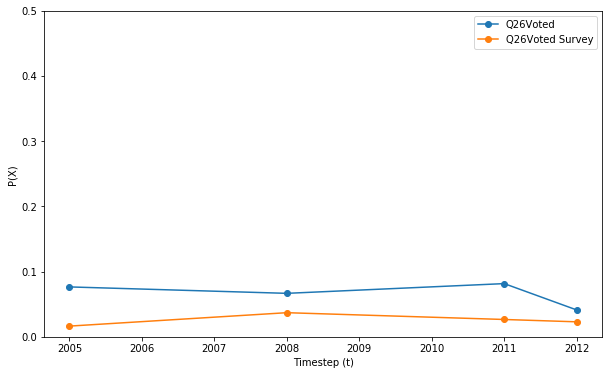
\includegraphics[width=0.7\linewidth]{Images/voted}
	\caption{}
	\label{fig:voted}
\end{figure}


%https://www.acleddata.com/dashboard/#800

\begin{figure}
	\centering
	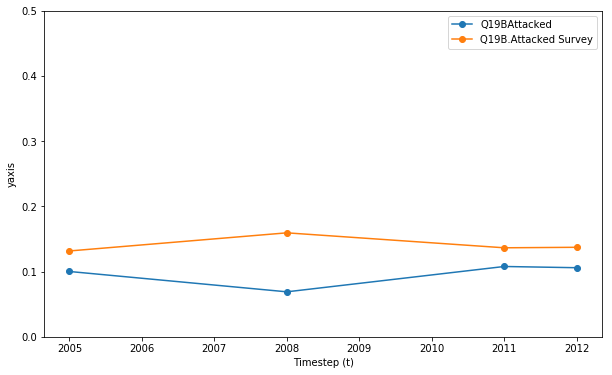
\includegraphics[width=0.7\linewidth]{Images/attacked}
	\caption{}
	\label{fig:attacked}
\end{figure}
\begin{figure}
	\centering
	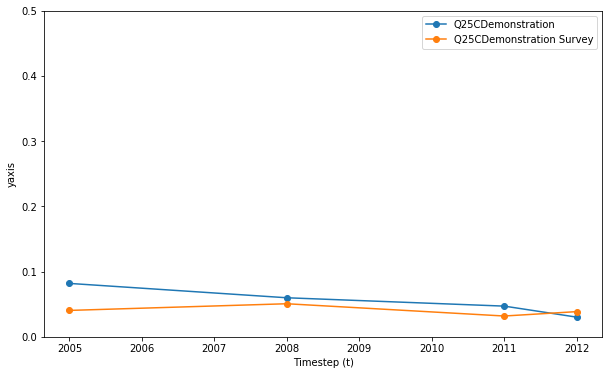
\includegraphics[width=0.7\linewidth]{Images/demonstration}
	\caption{}
	\label{fig:demonstration}
\end{figure}


\subsection{Model Verification}\label{sec:granularity}

An ideal model would be able to accurately model different scales of the survey participants with zero variance. Such universal model given as initial condition an individual's or group of participants current belief state would be able to determine the actions that they would take. Consequently, an ideal model design should be able to generate an ideal model. 

We set to verify that our model generation method can generate models that can scale. By generating a model $M_G$ from a set of survey participants $G$, we examine how well it models a superset or subset $G'$. We compare the outcome of predictions of $M_{G}(G)$ with $M_{G'}(G)$. We define our error as
\begin{eqnarray}
\varepsilon_{M} = |M_G(G) - M_{G'}(G)|
\end{eqnarray}

We use two approaches to evaluate how well the model scales, a bottom up approach and a top down approach. Consider a set $G$ for which we identify a set $\{g_1,..,g_n\}$ of participants that are an exact cover to the universal set $G$. Each disjoint subset $g_i$ has unique identifying characteristics such as age, sex, group affiliation. Consequently, $G=g_1\cup \cdots \cup g_n$ and $g_1\cap \cdots \cap g_n = \emptyset $. 

\subsubsection{Bottom-Up approach}\label{sec:bottomup}


We generate a model $M_{g_i} \forall g_i \epsilon G$. The motive is to demonstrate the how well the model fits a portion of the data it was trained on. To study this relation, we train a model $M_{g_i}$ on subset of the data and test it on the same subset. We train another model trained on dataset $G$ and train it on the subset $g_i$. Here $G$ is the superset of $g_i$. The error of $M_{g_i}$ is then:
\begin{eqnarray}
\varepsilon_{M_{g_i}}=|M_{g_i}(g_i)-M_{G}(g_i)|
\end{eqnarray}
The total error of the model evaluated through this approach is then given by:
\begin{eqnarray}
\varepsilon_{M_g} = \sqrt{\sum{\varepsilon_{M_{g_i}}}^2}
\end{eqnarray}


\subsubsection{Top-Down approach}\label{sec:topdown}
Similarly, we generate a model $M_{G}$ and $M_{g_i}$ for a subset $g_i\epsilon G$. The motive is to demonstrate the generalization capabilities of the model. We train a model $M_{g_i}$ on subset of the data and test it on the dataset $G$. We train another model $M_{G}$ on $G$ and test it on $G$. Here $G$ is the subset of $g_i$. he error is then given by:
\begin{eqnarray}
\varepsilon_{M_{G_i}}=|M_{G}(G)-M_{g_i}(G)|
\end{eqnarray}
The total error of the model evaluated through this approach is then given by:
\begin{eqnarray}
\varepsilon_{M_G} = \sqrt{\sum{\varepsilon_{M_{G_i}}}^2}
\end{eqnarray}

\subsubsection{Results}

\begin{table}
	
	\caption{Our Model Verification Results}
    \begin{center}
	\begin{tabular}{|l|l|l|l|l|}
		\hline
		& Statistic & P-Value & $\varepsilon_M$ & $\overline{W_p}(M(G_{M}),G_{{T}})$ \\
		
		\hline
		$M_{M}(G)$  &\multirow{2}{*}{0.231}&\multirow{2}{*}{0.828 }     &      \multirow{2}{*}{$7.878\cdot10^{-3}$}    & \multirow{2}{*}{$1.485\cdot10^{-2}$}   \\ 
		
		$M_{m}(G)$          &         &       & &              \\ 
		\hline
		
		$M_{M}(G)$          &   \multirow{2}{*}{ 0.153  }      &     \multirow{2}{*}{ 0.995}     &      \multirow{2}{*}{ $3.548\cdot10^{-3}$ }            & \multirow{2}{*}{$1.253\cdot10^{-2}$} \\ 
		
		$M_{f}(G)$         &           &        &  &  \\     
		
		\hline
		$M_{M}(G_{m})$          &   \multirow{2}{*}{0.0769 }      &     \multirow{2}{*}{$\sim1$}     &      \multirow{2}{*}{$7.413\cdot10^{-3}$}           & \multirow{2}{*}{$1.033\cdot10^{-2}$}\\ 
		
		$M_{m}(G_{m})$          &         &       & &             \\ 
		\hline
		
		$M_{M}(G_{f})$          &   \multirow{2}{*}{0.2308 }      &     \multirow{2}{*}{0.828 }     &      \multirow{2}{*}{$6.670\cdot10^{-3}$ }            & \multirow{2}{*}{$0.720\cdot10^{-2}$}\\ 
		
		$M_{f}(G_{f})$         &           &    &    &    \\     
		\hline
	\end{tabular}
	\end{center}
\end{table}

%The variance over time grows between the two models with different initial conditions and eventually stabilizes, which is to be expected due to the nature of a POMDP. We considered a timespan of 10 time steps for our visualizations, but evaluated only on the starting timesteps due to lack of observation updates as explained in  Section \ref{sec:observations}. 

For the top-down evaluation of the model's granularity Table \ref{tab:hdmtopdown} presents the results of statistical similarity. Mean variance is the difference between the two models set with the same initial states over all actions. 
%Figure \ref{fig:hdmvariance} visualizes the variance over time with each colored line representing the variance of that particular action. 

We evaluated using Kolmogorov–Smirnov statistical test on the probability distribution of the actions. Our results indicate that the $p$ value is larger than the statistic and we can't reject the null hypothesis, hence there is statistical similarity between the probability distributions generated by the two models. 


For the bottom-up evaluation of the model's granularity Table \ref{tab:hdmbottomup} presents the results of statistical similarity. Similarly as the top-down evaluation, the probability distributions generated by this method are statistically similar.

The conclusion of our results are that the variance is too small given the same initial conditions to consider that the model doesn't scale-down or scale-up well enough. Hence the model does provide a value at capturing different participants of the same population. 


\subsection{Model Evaluation}\label{sec:evaluation}

\begin{figure*}[t!]
	\centering 
	
\caption{Our Model Prediction over Time}
	\label{fig:groundtruth}
	\begin{minipage}{0.24\textwidth}
		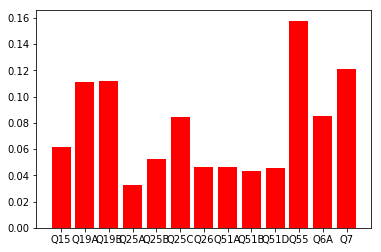
\includegraphics[width=\linewidth]{Images/pred_2005.png}
	\end{minipage}\hfill
	\begin{minipage}{0.24\textwidth}
		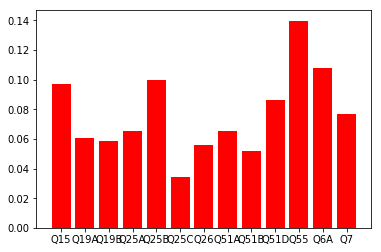
\includegraphics[width=\linewidth]{Images/pred_2008.png}
	\end{minipage}\hfill
	\begin{minipage}{0.24\textwidth}%
		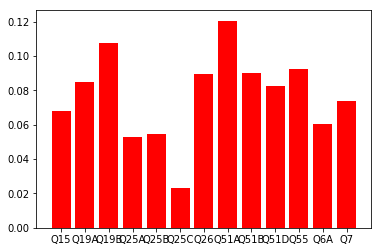
\includegraphics[width=\linewidth]{Images/pred_2011.png}
	\end{minipage}
	\begin{minipage}{0.24\textwidth}%
		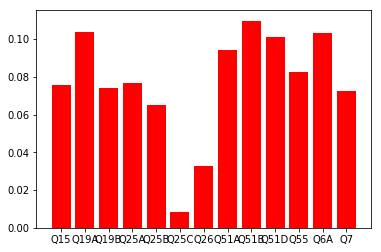
\includegraphics[width=\linewidth]{Images/pred_2012.png}
	\end{minipage}\\
	
	\caption{Survey Responses over Time}
	\begin{minipage}{0.24\textwidth}
		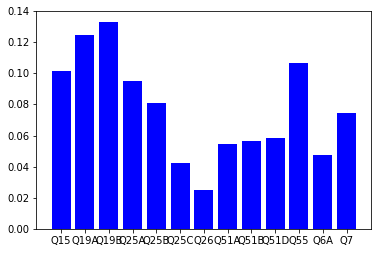
\includegraphics[width=\linewidth]{Images/true_2005.png}
	\end{minipage}\hfill
	\begin{minipage}{0.24\textwidth}
		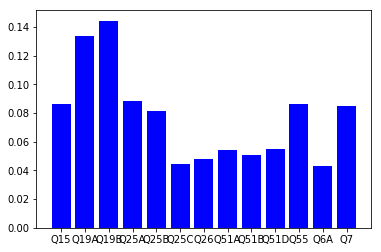
\includegraphics[width=\linewidth]{Images/true_2008.png}
	\end{minipage}\hfill
	\begin{minipage}{0.24\textwidth}%
		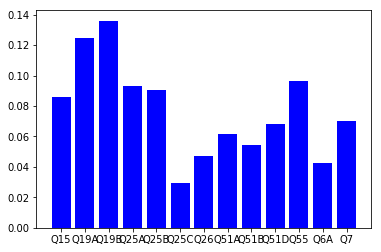
\includegraphics[width=\linewidth]{Images/true_2011.png}
	\end{minipage}
	\begin{minipage}{0.24\textwidth}%
		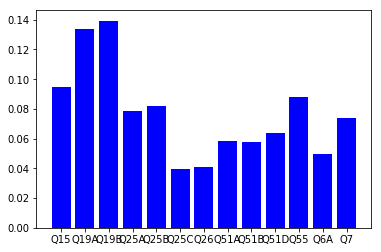
\includegraphics[width=\linewidth]{Images/true_2012.png}
	\end{minipage}\\
	
	\caption{Random Model Predictions over Time}
	\label{fig:predictions}
	\begin{minipage}{0.24\textwidth}
		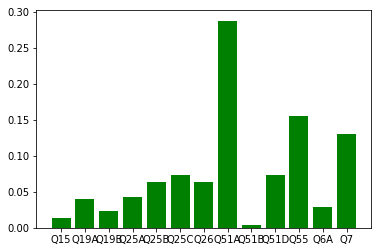
\includegraphics[width=\linewidth]{Images/random_pred_2005.png}
	\end{minipage}\hfill
	\begin{minipage}{0.24\textwidth}
		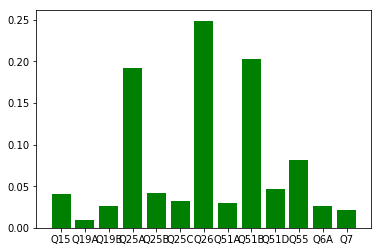
\includegraphics[width=\linewidth]{Images/random_pred_2008.png}
	\end{minipage}\hfill
	\begin{minipage}{0.24\textwidth}%
		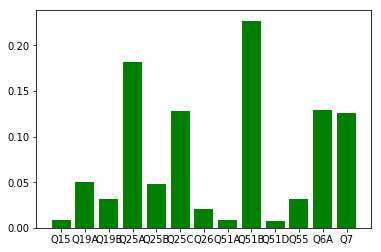
\includegraphics[width=\linewidth]{Images/random_pred_2011.png}
	\end{minipage}
	\begin{minipage}{0.24\textwidth}%
		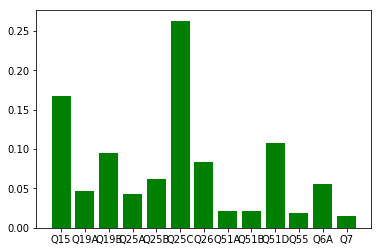
\includegraphics[width=\linewidth]{Images/random_pred_2012.png}
	\end{minipage}\\
	\label{fig:random}
\end{figure*}

We set to evaluate how well does our model compare to the actions that the participants actually take. For a set of survey participants, we split their responses into a model set, $G_M$ and a test set $G_T$. We used the model set to build a model out of them and then compare how similar the responses of that model were to the test set actions. We cross-validated using K-fold method with 10 folds. In order for the accurate comparison between the distributions we computed the mean for each action. The mean represents the probability that a participant will take that action based on sentiment strength as explained in Section \ref{sec:generatingdynamics}. The distribution of actions was then transformed to a normal distribution with sum of 1. 

We generate model $M$ from a set of participants $G_M$ and compute the difference between $G_T$. $G_M$ and $G_T$ are an exact cover of $G$.
\begin{eqnarray}
\varepsilon_{M}=|M(G_M) - G_T| 
\end{eqnarray}

Results of our model evaluation can be seen in Table \ref{tab:evaluation}, the distribution of actions and their difference at Figures \ref{fig:groundtruth} and \ref{fig:predictions}. Similar as the methodology in Section \ref{sec:bottomup}, we used Kolmogorov-Smirnov statistical test to compare the difference between the distribution and goodness of fit with statistically similar results. 



\begin{table}[!th]
	
	\caption{Our Model Evaluation Results}	
	\begin{tabular}{|l|l|l|}
		\hline
		& Statistic & $\overline{W_p}(M(G_{M}),G_{{T}})$\\
		
		\hline			
		$M(G_{2005})$    &      \multirow{2}{*}{ $3.395\cdot10^{-2}$ } & \multirow{2}{*}{$8.317\cdot10^{-3}$}            \\ 
		
		$M(G_{2005})$            & &   \\     
		\hline
		$M(G_{2008})$             &      \multirow{2}{*}{ $3.144\cdot10^{-2}$ }  &  \multirow{2}{*}{$1.060\cdot10^{-2}$}         \\ 
		
		$M(G_{2008})$                &   & \\     
		\hline
		$M(G_{2011})$           &      \multirow{2}{*}{ $3.144\cdot10^{-2}$ }    & \multirow{2}{*}{$1.127\cdot10^{-2}$}          \\ 
		
		$M(G_{2011})$            &    &\\     
		\hline	
		
		$M(G_{2012})$              &      \multirow{2}{*}{ $4.268\cdot10^{-2}$ }    &     \multirow{2}{*}{$1.400\cdot10^{-2}$}       \\ 
		
		$M(G_{2012})$           &   & \\     
		\hline						
	\end{tabular}\label{tab:evaluation}

\end{table}

\subsection{Baseline Model}\label{sec:random}

Using the results from section \ref{sec:evaluation}, we set out to examine how well our model compares to a baseline. Due to lack of a baseline from previous works, we compare our error with that of a Random Model Design. We define a Random Model $M_{R_G}$ as a model generated by taking an existing model $M_G$ and modifying the rewards, priorities and impact of actions in a random manner. The overall structure and connection of the model are not changed. We aim to test if a Random Model is able to evaluate better than our current model. 

Consequently, we generate model $M_{R_G}$ with Random dynamics from a set of participants $G_M$ and compute the difference between $G_T$ and $M_{R_G}$. $G_M$ and $G_T$ are an exact cover of $G$.

the calculation of the Random Model error is:
\[\varepsilon_{M_{R_G}}= | M_{R_G}(G)-G_T |\] 

We run on the same parameters and initial conditions as section \ref{sec:evaluation} and we compare our results. We cross-validate again with K-Fold K=10. The results are presented in Table \ref{tab:random}. It can be confirmed by comparison with \ref{tab:evaluation} that the average  Wasserstein Distance, $\overline{W_p}$  between the Random population and the Survey values is in almost double in most cases than our own model's prediction values. The result can be verified visually by comparing Figure \ref{fig:random} with Figure \ref{fig:groundtruth}.

\begin{table}[!th]
	
	\caption{Random Model Results}
	\begin{tabular}{|l|l|l|}
		\hline
		& Statistic & $\overline{W_p}(M(G_{M}),G_{{T}})$\\
		
		\hline			
		$M(G_{2005})$    &      \multirow{2}{*}{ $3.462\cdot10^{-2}$ } & \multirow{2}{*}{$2.266\cdot10^{-2}$}            \\ 
		
		$M(G_{2005})$            & &   \\     
		\hline
		$M(G_{2008})$             &      \multirow{2}{*}{ $4.126\cdot10^{-2}$ }  &  \multirow{2}{*}{$3.462\cdot10^{-2}$}         \\ 
		
		$M(G_{2008})$                &   & \\     
		\hline
		$M(G_{2011})$           &      \multirow{2}{*}{ $3.985\cdot10^{-2}$ }    & \multirow{2}{*}{$1.127\cdot10^{-2}$}          \\ 
		
		$M(G_{2011})$            &    &\\     
		\hline	
		
		$M(G_{2012})$              &      \multirow{2}{*}{ $2.936\cdot10^{-2}$ }    &     \multirow{2}{*}{$1.400\cdot10^{-2}$}       \\ 
		
		$M(G_{2012})$           &   & \\     
		\hline						
	\end{tabular}
	\label{tab:random}
\end{table}

\section{TESTING HYPOTHESES}

The generated models were tested with two kinds of hypotheses. First, we wanted to confirm the model generation process for a particular agent which can be an individual,tribe or country. We picked a sample to be an agent from the tribe Muganda Uganda from year 2005. The sample was chosen because of its decent response represenation in data. The model was generated for the agent \textit{A}. To study if the model is able to generate similar distribution for an agent \textit{A'}, whose prior belief of the environment belief state in study in zero. We then generate a model for \textit{A'}, after running simulation with the agent environment learned from model of \textit{A}. The resulting distribution of actions for \textit{A'} was similar to \textit{A} for a belief state with initial value set to zero for \textit{A'}. We repeated the same process for different belief states, yielding similar results, the model generated for both agents had similar probability distribution. This concludes the first hypotheses that the model is able to generate similar behavior for a new agent introduced to an agent environment.


\begin{table}[!th]
	
	\caption{Probability Distribution Entropy Increase }
	\begin{tabular}{|l|l|}
		\hline
	$ Hypotheses$	& KL-Divergence($A$,$A'$) \\
		
		\hline			
		$ Living\_Conditions$    &     0.0007097       \\ 
		
		       
		\hline
		$ No\_water$             &      0.0016947       \\ 
		
		    
		\hline
		$ Being\_Attacked $          &     0.0053039        \\ 
		
		    
		
		    
		\hline						
	\end{tabular}
	\label{tab:random}
\end{table}

After establishing the generation of similar behavior, it was important to test if the behavior generated for a belief state was indeed what can be expected in a given situation and not something generated arbitrarily. The second hypotheses was testing the behavior of agent \textit{A'} for different belief states. We tested the model against living conditions, lack of water and being attacked recently.  For belief states 'living conditions' and 'lack of water', 'education' came out to be as probable action for \textit{A'}, with slightly higher probability than what was seen for agent \textit{A}. While there is no data recording the desire of people to pursue education, the model behavior could be framed by a simple heuristic, the number of people with NOT poor living conditions and NOT lack of water are educated to some level of qualification. Affirmatively, when tested for the belief state 'being attacked', the model responded with a slightly lower probability for 'education' than what was seen for \textit{A}, while probability was high for 'something stolen' and 'president ignores the situation'. Interestingly, the probability was low for actions like 'competition' and 'employment', which confirms that the model is not generating similar arbitrary behaviors.

The results described in Table.5 are for actions Education E, President\_Ignores\_Situation PI, Something\_Stolen SS, Competition C and Employment EMP. 
 
\begin{table}[!th]
	
	\caption{Hypotheses-Action Probabilities }
	\begin{tabular}{|l|l|l|l|l|l|}
		\hline
	$ Hypotheses/Actions$	& E & PI & SS & C & EMP \\
		
		\hline			
		$ Living\_Conditions$    &     0.0622 & 0.0829 & 0.056 & 0.033 & 0.037        \\ 
		
		       
		\hline
		$ No\_water$             &      0.0657 & 0.0773 & 0.0618 & 0.0340 & 0.0348       \\ 
		
		    
		\hline
		$ Being\_Attacked $          &     0.0540 & 0.0922 & 0.0764 & 0.0331 & 0.0349         \\ 
		
		    
		
		    
		\hline						
	\end{tabular}
	\label{tab:random}
\end{table}
 
\section{DISCUSSION}

The model generated by this design has value in generating a behavior model from  survey data. We minimize the human input required to that of identifying and mapping survey questions to pre-defined abstractions build on top of a POMDP model. During the model implementation phase we minimize the bias that can be added by the model user and aid in a more automated approach at constructing a behavior model. Moreover other researchers that utilize this approach to generate a behavior model, don't require complete domain knowledge of the subjects they are studying. 

The results show that the model design we have chosen can scale between representing multiple demographics with one model. We present a baseline of performance for our behavior model and an evaluation method. The results of this paper can be used in the future to optimize the behavior model and generate even more complex dynamics that encapsulate social interactions even more accurately.

We seek to continue evaluating and improving the model on surveys and experiments specifically designed to capture the elements that would give better insight on the behavior of the study subjects. We seek to evaluate it on more complex scenarios where we consider the observations and updated dynamic states during a simulation. 

In the future we are considering expanding a version of this model design to further automate the link between data and the construction of a behavior model to consider additional formats of input with the same objective. The model design inherently is not limited to survey data and we could perform similar experiments with the right data analysis pipeline. 
 
Human bias in the selection of actions and dynamic states can be transferred in the final model. For our evaluation we selected what we considered to be valid actions by inferring from the survey data and hence this bias is build into the evaluation of our approach. 


\section{CONCLUSION}
In this work, we showed the automated generation of human behavior model leveraging statistical correlations among variables of a POMDP with minimal manual design choices. Even though, it is not conclusive from the statistical correlation itself the existence of a causal model from the data, our automatically generated model was able to capture certain  trends in responses and behavior that resonated with the data. We showed a way of testing different hypotheses in such setup and how these hypotheses could be used to validate model behavior.

Due to unavailability of a baseline model performance on the data, we set out to test our model against a randomly set model with same variables as our model. This helped illustrate that our automated generation of a model with minimal manual intervention outperforms a randomly generated model in learning behaviors. Our model also demonstrates support for modeling subjects at different level of granularity, i.e individual,tribe,gender, country, with minimal human intervention.

We also set out to test the generalization capabilities of the model. This was demonstrated by the Top-Down approach of model evaluation. The results show that the model is able to generalize to the data coming from a similar distribution, capturing behavior based on granularity (i.e an individual, tribe, gender etc).

We also tested the model's power of learning through statistical correlations by comparing the model's probability distribution over variables on train set and test set. Since, we can't reject the null-hypothesis, the probability distributions generated for the two sets were similar. This leads to conclude that the model is able to capture subject's behavior to some extent.




%%%%%%%%%%%%%%%%%%%%%%%%%%%%%%%%%%%%%%%%%%%%%%%%%%%%%%%%%%%%%%%%%%%%%%%%%%%%%%%%%%%%%%%%%%%%%%%%%%%%%%%%%
%% bibliography: see CFP for number of permitted pages

\bibliographystyle{ACM-Reference-Format}  % do not change this line!
\bibliography{bibliography}  % put name of your .bib file here

\end{document}
